%!TEX root = ../main.tex

\subsection{Compiling Specifications to Parametrised Tests}

\subsection{Example} 

In general, the specification of a given library must ensure that all prototype chains are consistent with correct library behaviour by stating which resources must not be present for its code to run correctly.
In particular, constructed objects cannot redefine properties that are to be found in their prototypes;  and prototypes cannot define as \emph{non-writable} those properties that are to be present in their instances. 
We refer to these two criteria as \emph{prototype safety}, and illustrate how it can be achieved through the specification of the key-value map. 

We define a \emph{map object predicate} below, \jsinline|Map|, using the auxiliary 
predicate \jsinline|KVPairs|, which captures the resource of the key-value pairs in the map, 
and the \jsinline|validKey(k)| predicate, which holds if and only if the JavaScript function \jsinline|ValidKey(k)| returns \jsinline|true|\footnote{We treat the $\mathtt{ValidKey}$ predicate as a black box, other than requiring that $\mathtt{hasOwnProperty}$ is not a valid key.}.
%
Intuitively, the \jsinline|Map(m, mp, kvs, keys)| predicate captures the resource 
of a map object \jsinline|m| with prototype \jsinline|mp|, keys \jsinline|keys| (a set of strings),
and key-value pairs \jsinline|kvs| (a set of string pairs\footnote{We model pairs as lists with two elements and, for clarity, use the pair notation.}).  
%
The definition of \jsinline|Map| achieves the first requirement for prototype safety by stating that a 
map object \jsinline|m| cannot have the properties \jsinline|"get"|, \jsinline|"put"|, and \jsinline|"validKey"|, and that the 
object bound to \jsinline|_contents| cannot have the property \jsinline|"hasOwnProperty"|. 
The \jsinline|emptyFields| predicate, together with the prototype safety requirement \jsinline|(c, "hasOwnProperty") ->  None|, ensures that there are no other properties in the contents of the map except the keys.
%
We write \jsinline|-u-| for set union and omit the brackets around singleton 
sets when the meaning is clear from the context. 
%\pg{I would put map before KVPairs, its' the one I went to first.}
\vspace{3pt}
\begin{center}
{\footnotesize
 \begin{verbatim}
Map (m, mp, kvs, keys) := JSObject(m, mp) * 
  DataProp(m, "_contents", c) * JSObject(c, Object.prototype) * 
  (m, "get") -> None * (m, "put") ->  None * (m, "validKey") ->  None * 
  (c, "hasOwnProperty") ->  None * KVPairs(c, kvs, keys) * emptyFields(c, keys -u- "hasOwnProperty")
  \end{verbatim}
  \vspace*{-0.3cm}
 \begin{verbatim}
KVPairs (o, kvs, keys) := 
  (kvs = { }) * (keys = { }),
  (kvs = (key, value) -u- kvs') * (keys = key -u- keys') * 
    ValidKey(key) * DataProp(o, key, value) * KVPairs(o, kvs', keys')
\end{verbatim}}
\end{center}

Observe that the definition of \jsinline|Map| does not include the resource of a map prototype. 
As \jsinline|Map.prototype| is shared between all map objects, we cannot include the resource of a map prototype 
in the definition of \jsinline|Map|. Were we to do that, we could no longer write a satisfiable assertion 
describing two distinct map objects using the standard separating conjunction.
Below, we show the definition of \jsinline|MapProto|, stating that a valid map prototype has the properties 
\jsinline|"get"|, \jsinline|"put"|, and \jsinline|"validKey"|, respectively assigned to the appropriate functions (see~\S\ref{subsec:absbasic}). 
The definition of \jsinline|MapProto| achieves the second requirement for prototype safety by stating that a 
map prototype cannot have the property \jsinline|"_contents"|. We could have weakened this definition, stating that 
a map prototype can have the property \jsinline|"_contents"|, as long as it is writable. 
In Figure~\ref{fig:objmap}, we give a graphical representation of the assertion
\jsinline|Map (m, mp, kvs, keys) * MapProto (mp)|.
\vspace{3pt}
\begin{center}
{\footnotesize
 \begin{verbatim}
MapProto (mp) :=  JSObject(mp, Object.prototype) * (mp, "_contents") -> None) * 
   DataProp(mp, "get", gf)       * FunctionObject(gf, "get", g_sc) * 
   DataProp(mp, "put", pf)       * FunctionObject(pf, "put", p_sc) * 
   DataProp(mp, "validKey", vkf) * FunctionObject(vkf, "validKey", vk_sc) 
\end{verbatim}}
\end{center}
%\pg{Remind reader about function objects and function identifiers, just lightly.}

\begin{figure}[t]
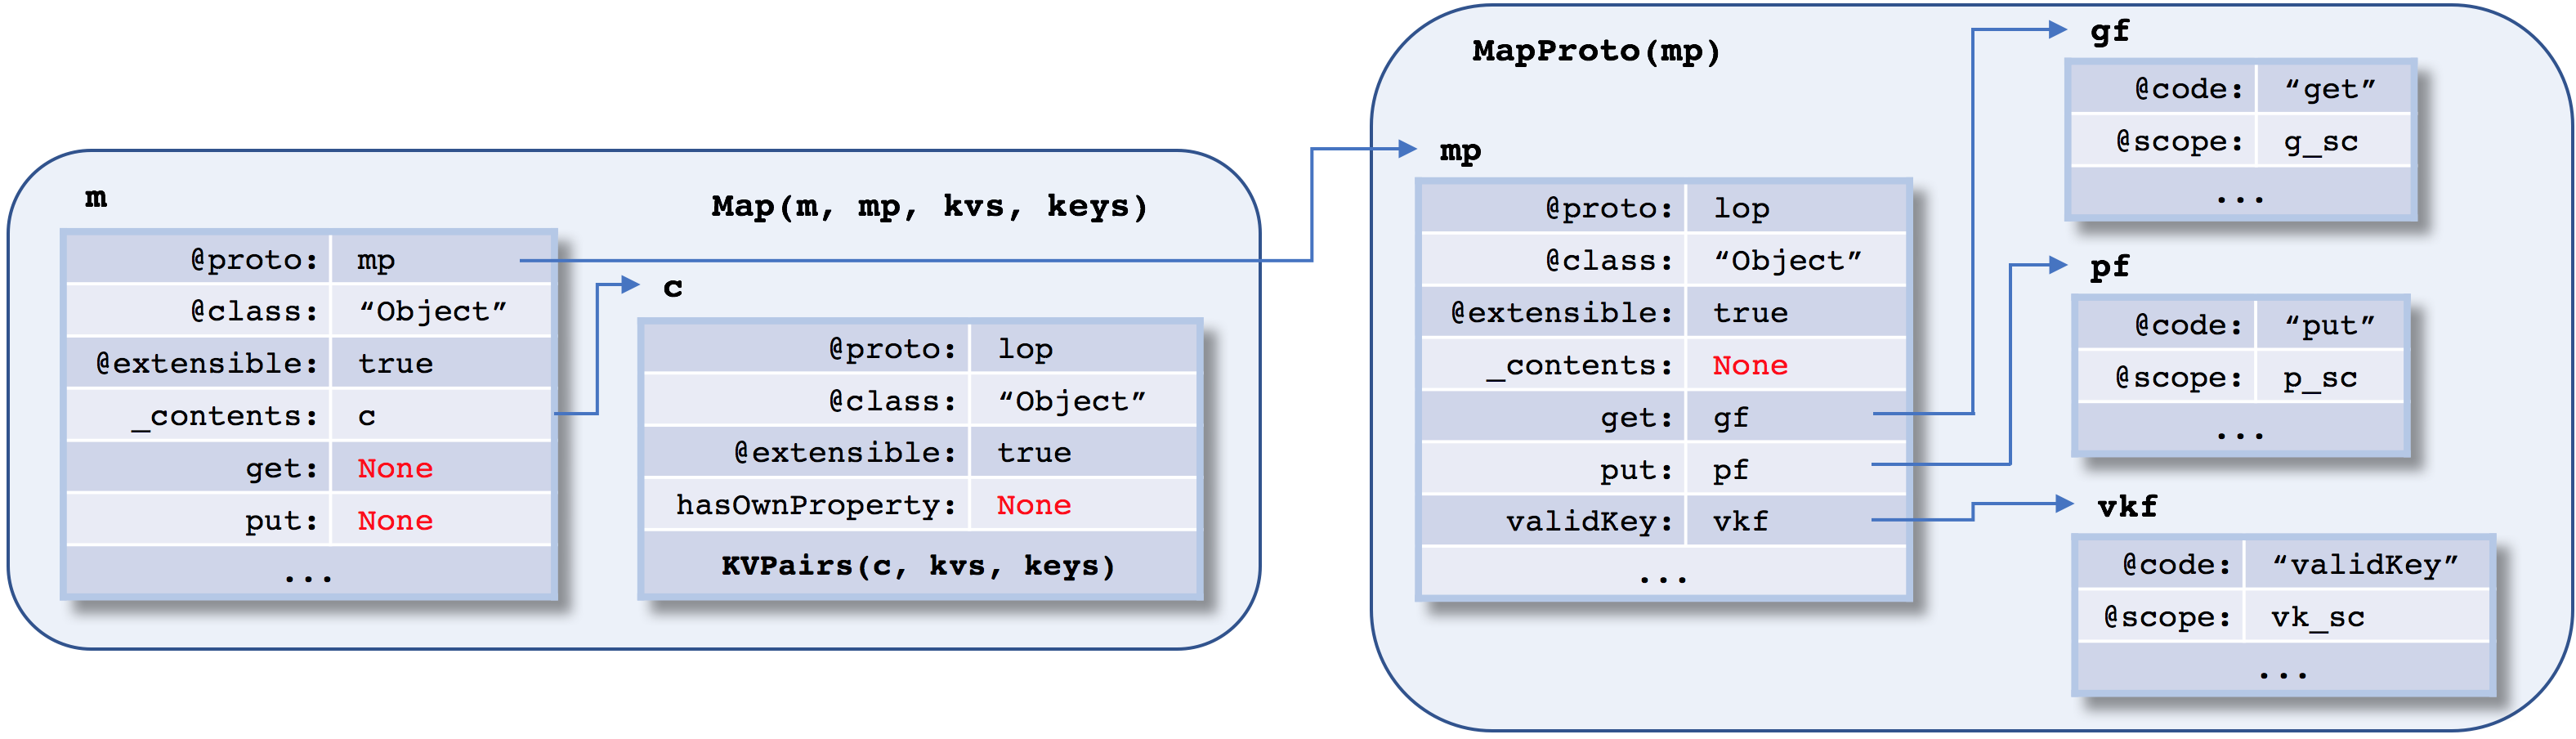
\includegraphics[width=0.95\textwidth]{figures/objectAsMap.png}
\vspace*{-0.2cm}
\caption{Graphical representation of
\jsinline|Map (m, mp, kvs, keys) * MapProto (mp)|}
\label{fig:objmap}
\vspace*{-0.3cm}
\end{figure}



We are now in the position to specify the functions of the map library. In particular, below we show how to use 
the map object predicate and the map prototype predicate to specify \jsinline|put(k, v)|.  
%
The first specification captures the case in which the key of key-value pair to be inserted 
already exists in the map, while the second one captures the case in which it does not. 
The third specification captures the error case, when the given key is not valid.
Since \jsinline|put| calls the function \jsinline|validKey|, all of its specifications must include the \jsinline|MapProto(mp)| predicate, that captures the location of \jsinline|validKey|. 

\noindent

\begin{displaymath} 
{\footnotesize
\begin{array}{c}
\left\{ {\begin{array}{c}
 \text{\texttt{Map(this, mp, kvs -u- (k, v'), ks) *}} \\ 
 \text{\texttt{MapProto(mp) * ObjProtoF()}} 
\end{array}} \right\} \\
%
\text{\bfseries \texttt{put(k, v)}} \\[0.2mm]
%
\left\{ {\begin{array}{c}
 \text{\texttt{Map(this, mp, kvs -u- (k, v), ks) *}} \\
 \text{\texttt{MapProto(mp) * ObjProtoF()}} 
\end{array}} \right\}
\end{array}
} 
\end{displaymath}


\begin{displaymath} 
{\footnotesize
\begin{array}{c}
\left\{ {\begin{array}{c}
 \text{\texttt{Map(this, mp, kvs, ks) * MapProto(mp) *}} \\
 \text{\texttt{!(k -in- ks) * ValidKey(k) * ObjProtoF()}} 
\end{array}} \right\} \\
%
\text{\bfseries \texttt{put(k, v)}} \\[0.2mm]
%
\left\{ {\begin{array}{c}
 \text{\texttt{Map(this, mp, kvs -u- (k, v), ks -u- k) *}} \\
 \text{\texttt{MapProto(mp) * ObjProtoF()}} 
\end{array}} \right\} \\
\end{array}}
\end{displaymath}

\begin{displaymath} 
{\footnotesize
\begin{array}{c}
\left\{ {\begin{array}{c}
 \text{\texttt{Map(this, mp, kvs, ks) * MapProto(mp) * !ValidKey(k) * ObjProtoF()}} 
\end{array}} \right\} \\
%
\text{\bfseries \texttt{put(k, v)}} \\[0.2mm]
%
\left\{ {\begin{array}{c}
 \text{\texttt{Map(this, mp, kvs, ks) * MapProto(mp) * ErrorObject(err) * ObjProtoF()}} 
\end{array}} \right\}
\end{array}
} 
\end{displaymath}

Recall that the prototype safety requirements of the library extend to \jsinline|Object.prototype| as well. 
This resource is captured by the built-in \jsinline|ObjProtoF()| predicate, describing the frozen
\jsinline|Object.prototype| object (see \S\ref{subsec:absbasic}). Here, the user can instead choose to use the open version of the predicate, \jsinline|ObjProto()|, allowing for a more flexible initial heap. In that case,
they would have to manually specify the prototype safety requirements, as we have done for maps and the map prototype.

